% !TeX spellcheck = ru_RU
% !TEX root = vkr.tex

\section{Обзор}

Данный раздел содержит обзор сущностей, взаимодействующих с глобальной очередью, инструментов бенчмаркинга.

\subsection{Асинхроное замыкание}

Далее представлен код демонстрирующий описание асинхронного замыкания:

\begin{listing}[H]
    \begin{minted}{rust}
let closure =  async {
    tokio::time::sleep(Duration::from_secs(10)).await;
}
    \end{minted}

    \caption{Асинхронное замыкание}
    \label{listing:async_closure}
\end{listing}

Значениие связанное с именем \verb|closure| имеет представляет собой конечный автомат, ожидающуй 10 секунд, и реализует следующий тип:

\begin{listing}[H]
    \begin{minted}{rust}
trait Future {
    type Output;
    fn poll(self: Pin<&mut Self>, cx: &mut Context)
        -> Poll<Self::Output>;
}
    \end{minted}

    \caption{Асинхронное замыкание}
    \label{listing:future_trait}
\end{listing}

Где метод \verb|poll| выражает попытку совершить переход от состояния к состоянию и сигнализиует о завершении выполнения всего замыкания с помощью слеюущего типа:

\begin{listing}[H]
    \begin{minted}{rust}
    pub enum Poll<T> {
        Ready(T),
        Pending,
    }
    \end{minted}

    \caption{Асинхронное замыкание}
    \label{listing:future_trait}
\end{listing}

То есть возвращает вариант \verb|Ready| с результирующим значением в случае заверешения и \verb|Pending| в противном случае.

Метод \verb|poll| в качестве первого аргументы принимает само асинхронное замыкание, окруженного структурой \verb|Pin| --- это необходимо для статической гарантии безопасности. В качестве второго аргументы принимает контекст, который прежде всего служит для регистрации значения \verb|Waker|, связывающего асинхронные замыкания.

Структура \verb|Waker| имеет метод wake() призванный уведомить о годовности замыкания совершать прогресс, если сейчас оно еще не готово, то есть вернуло Pending.

\subsection{Интерфейс tokio}

В следствии выше сказанного любое асинхронное замыкание можно исполнить достатчно долго вызывая на нем метод \verb|poll|. Однако, для удобства и эффективности использования асинхронного интерфейса предоставляемого языком Rust проект tokio предоставляет собственный интерфейс для исполнения асинхронных замыканий, среди которого метод \verb|tokio::spawn| регистрирующий асинхронное замыкание на исполнение в рантайме tokio и возвращающий значение \verb|JoinHandle| позволяющее ожидать исполнение исходного замыкания, получить результирующее значение или отменить исполнение вовсе. Например, исполнить представленное выше замыкание можно следующим образом:

\begin{listing}[H]
    \begin{minted}{rust}
let join_handle = tokio::spawn(async {
    tokio::time::sleep(Duration::from_secs(10)).await;
})
while !join_handle.is_finished() {}
    \end{minted}

    \caption{Ожидание исполнения асинхронного замыкания}
    \label{listing:tokio_spawn::sleep}
\end{listing}

\subsection{Жизненный цикл задачи}

\subsubsection{Создание задачи}

Обработка асинхронного замыкания переданного пользователем в метод \verb|tokio::spawn| начинается со следующего:

\begin{itemize}
    \item Создание уникального индентификатора задачи. Просиходит это с помощью статической атомарной переменной над которой выполняется FAA с relaxed семантикой.
    \item Процесс аллокации на куче структуры содержащей замыкание, счетчик указателей, результирующее значение и другие служебные инварианты, так называемой \verb|Cell| на куче.
    \item Созданием трех указатейлей на эту область памяти: \verb|Task|, \verb|Notified| и \verb|JoinHandle|.
    \begin{itemize}
        \item \verb|Task| сразу после создания добавляемым в OwnedQueue --- очередь предназначенную для хранений указателей на все задачи в данный момента аллоцированные рантаймом.
        \item \verb|Notified| является единицей шедулинга и сразу после созданий отпарвляется в шедулер tokio рантайма.
        \item \verb|JoinHandle|, как было сказано выше, является пользовательской структурой взаимодейсвия с задачей внутри tokio рантайма.
    \end{itemize}
\end{itemize}

\subsubsection{Исполнение задачи}

После чего, происходит процесс исполнения задачи: каждый раз, когда асинхронное исполнение готово совершать прогресс, создается структура Notified, отправляемая в шедулер tokio рантайма. При исполнении которой вызывается метод \verb|poll|, деаллокцирующий значение Notified, косвенно исполняющий метод \verb|poll| на исоходном замыкании.

Таким образом по говотовности каждого асинхронного замыкания уже аллоцированного tokio рантаймом создается указатель Notified отправляемый на исполнение в шедулер.

\subsubsection{Удаление задачи}

При достижении конечного состояни \verb|Task| удаляется из \verb|OwnedQueue| а \verb|Cell| деаллоцируется.

\subsection{Шедулер многопоточного рантайма tokio}

При инстанциации рантайм создает определенное количество системных потоков для так называемого блокирующего пулла, призванного исполнять ресурсоемкие задачи. Всего создается \verb|worker_threads| + \verb|max_blocking_threads| потоков, где

\begin{itemize}
    \item \verb|worker_threads| --- количество потоков предназначенных для исполнения асинхронных задач
    \item \verb|max_blocking_threads| --- максимальное количество блокирующих потоков
\end{itemize}

\begin{figure}[H]
    \begin{center}
        \makebox[\textwidth]{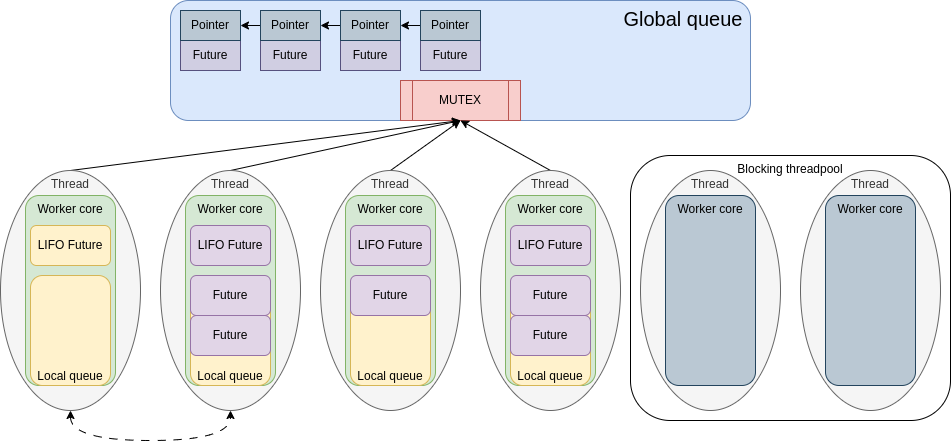
\includegraphics[scale=0.55]{pictures/tokio.arch.png}}
    \end{center}

    \caption{Упрощенное представление многопоточного рантайма}
    \label{fig:tokio:arch}
\end{figure}

Блокирующие потоки ожидают определенный период, 10 секунд если не специфицировано иначе, поступления задач после чего прекращают свое исполнение.

\verb|Воркер|, так называется сущность ассоциированная с каждым из оставшихся \verb|worker_threads| потоков с помощью размещения в локальной для этих поток переменной так называемого \verb|ядра воркера| --- структуры, необходимой для исполнения асинхронных задач, включающей \verb|локальную очередь|, хендлер \verb|глобальной очереди| и тому подобное.

\verb|Локальная очередь| воркера выступает в качестве кэша его Notified задач, имеет фиксированный размер и предполагает добавление задач исключительно из потока владельца. Однако, изъятие из нее может быть осуществлено потоками других воркеров при нехватке воркеру Notified задач --- процесс называемый стилингом. Все это: фиксированный размер и производитель в единственном количестве позволяет ей иметь lock free алгоритм взаимодействия. В случае переполнения часть задач перемещается в глобальную очередь.

\verb|Глобальная очередь| или \verb|inject queue| представляет собой коллекцию Notified задач ожидающих исполнения. Наполняется она при спавнинге задачи вне контекста воркера или при переполнении локальной очереди. Реализована с помощью интрузивного связного списка, защищенного мьютексом.

\subsubsection{Выбор задачи воркером}

Логика поиска воркером задачи для исполнения отражена на листинге \ref{listing:next_task}.

\begin{listing}[H]
    \begin{minted}{rust}
fn next_task(&mut self) -> Option<Notified> {
    if self.tick % self.global_queue_interval == 0 {
        return next_remote_task()
                .or_else(|| self.next_local_task())
    }
    if Some(task) = self.next_local_task()  {
        return Some(task);
    }
    if inject().is_empty() {
        return None;
    }
    let (head, tail) = inject().pop_n(self.can_take());
    self.run_queue.push_back(tail);
    return head
}
    \end{minted}

    \caption{Логика выбора задачи}
    \label{listing:next_task}
\end{listing}

И осуществляется в следующем порядке: раз в определенное, конфигурируемое рантаймом, число тиков --- мера времени воркера, он пытается взять задачу из глобальной очереди, иначе --- из локальной, в остальное время проверке подлежит локальная, после --- глобальная очереди.

\subsubsection{Цикл работы воркера}

Алгоритм рабочего цикла воркера отражен на листинге \ref{listing:worker:run}.

\begin{listing}[H]
    \begin{minted}{rust}
fn run() {
    while !is_shutdown() {
        core.tick();
        if let Some(task) = core.next_task() {
            self.run_task(task, core);
            continue;
        }
        if let Some(task) = core.steal_work() {
            self.run_task(task, core);
            continue;
        }
        self.park(core)
    }
}
    \end{minted}

    \caption{Логика выбора следующей задачи}
    \label{listing:worker:run}
\end{listing}

А именно, воркер отсчитывает тик, затем пытается найти задачу, после чего пытается украсть задачи у других воркеров. В случае неудачи он паркует поток.

\subsection{Бенчмаркинг}

Для измерений производительности была использована библиотека \verb|criterion|\footnote{\href{https://github.com/bheisler/criterion.rs}{Репозиторий} проекта criterion (Дата обращения: 4.1.2025)}. Так как она популярна, имеет обширную документацию и используется в \verb|tokio|.
